\subsection{Chapter Overview}

\subsection{Experimentation Setup}

\begin{figure}[H]
\centering
\graphicspath{ {./images/} }
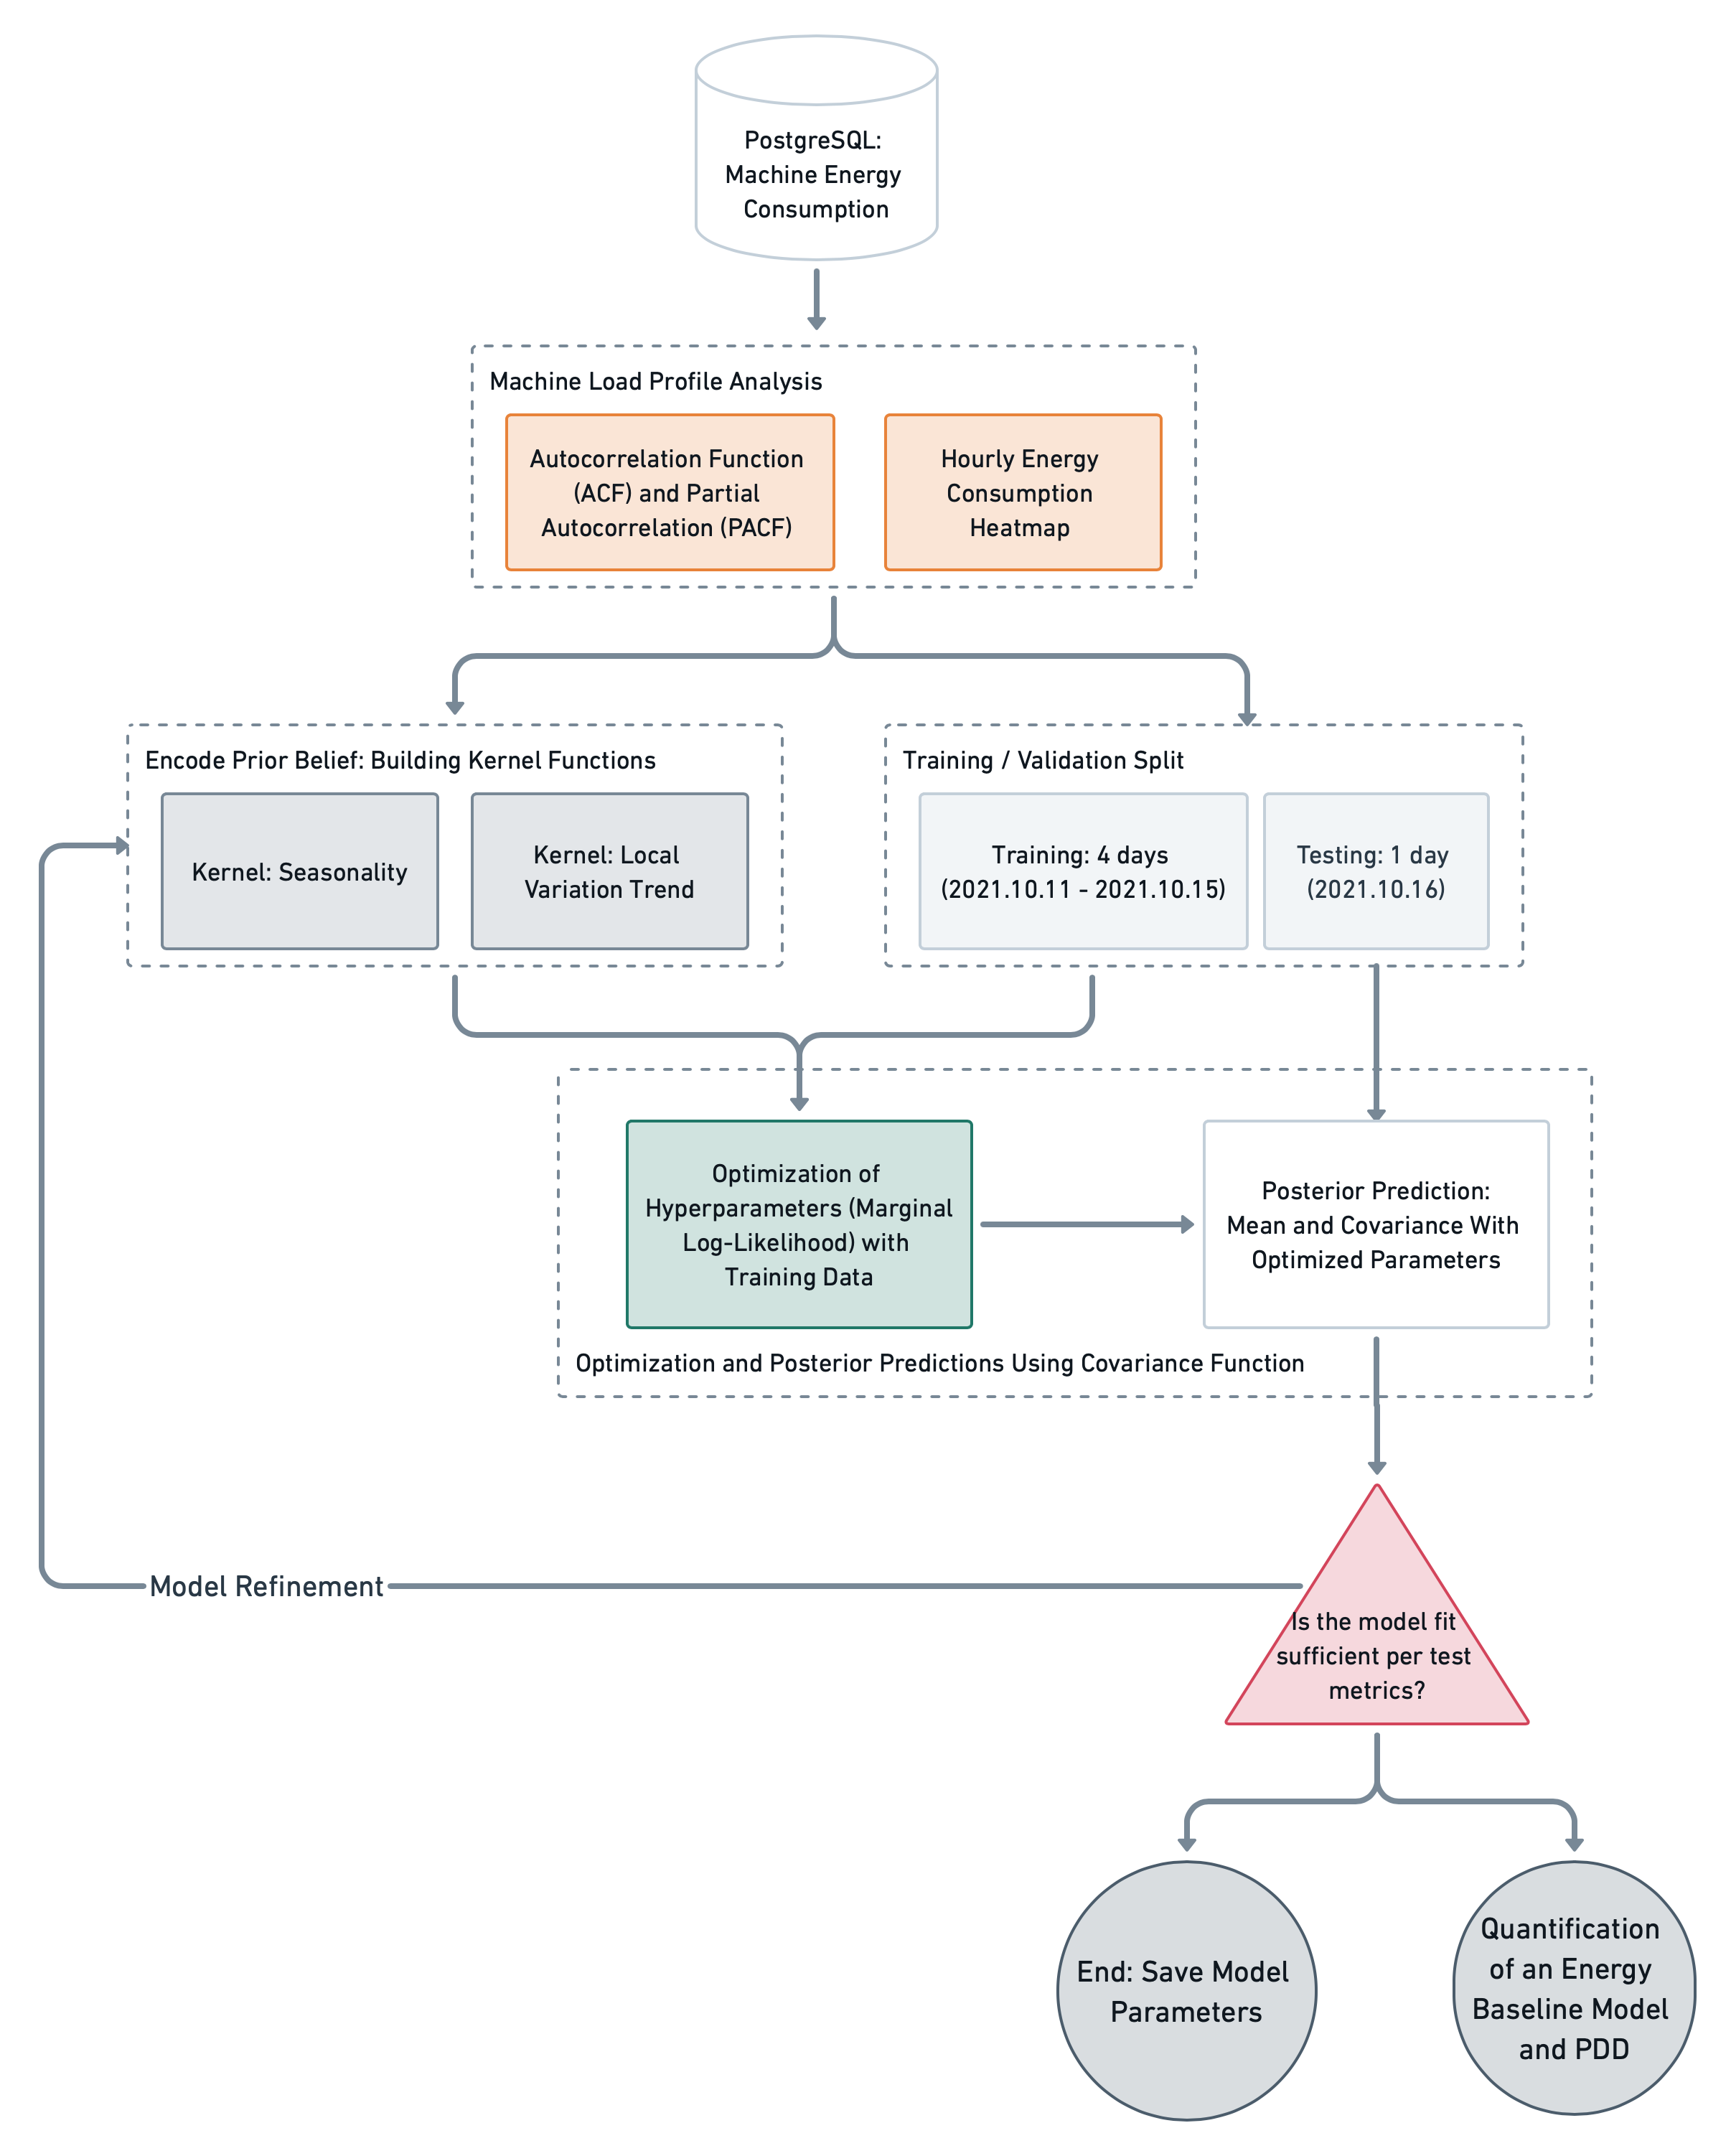
\includegraphics[scale=0.17]{images/experiment_flow.png}
\caption{Experimentation workflow for developing and refining GP energy baseline models.}
\end{figure}

\subsection{Model and Kernel Design, and Kernel Composition}

\subsection{Model Design Decomposition}

\subsection{Optimization and Cross Validation}

\subsection{Energy Baseline Model Experiment Performance Metrics}

\hyperlink{table.3}{Table 3} below shows

\begin{table}[htbp]
    \renewcommand{\arraystretch}{1.2}
    \centering
    \begin{tabular}{lcccccccc}
    \hline
         Device & Aggregation & Kernel & MSE & MAPE & RMSE & ACE & Pinball  \\
    \hline
    Paper disposal & $10$ & $K_{LocPer} + K_{RQ}$ & $0.155$ & $0.017$ & $0.39$ & $1.0$ & $0.145$ \\
     & $30$ & $K_{LocPer} + K_{RQ}$ & $0.155$ & $0.017$ & $0.39$ & $1.0$ & $0.145$ \\
    Gesamtmessung & $10$ & $K_{LocPer} + K_{RQ}$ & $0.155$ & $0.017$ & $0.39$ & $1.0$ & $0.145$ \\
     & $30$ & $K_{LocPer} + K_{RQ}$ & $0.155$ & $0.017$ & $0.39$ & $1.0$ & $0.145$ \\
    eg & $10$ & $K_{LocPer} + K_{RQ}$ & $0.155$ & $0.017$ & $0.39$ & $1.0$ & $0.145$ \\
     & $30$ & $K_{LocPer} + K_{RQ}$ & $0.155$ & $0.017$ & $0.39$ & $1.0$ & $0.145$ \\
    Hauptluftung & $10$ & $K_{LocPer} + K_{RQ}$ & $0.155$ & $0.017$ & $0.39$ & $1.0$ & $0.145$ \\
     & $30$ & $K_{LocPer} + K_{RQ}$ & $0.155$ & $0.017$ & $0.39$ & $1.0$ & $0.145$ \\
    og 1 & $10$ & $K_{LocPer} + K_{RQ}$ & $0.155$ & $0.017$ & $0.39$ & $1.0$ & $0.145$ \\
     & $30$ & $K_{LocPer} + K_{RQ}$ & $0.155$ & $0.017$ & $0.39$ & $1.0$ & $0.145$ \\
    uv eg & $10$ & $K_{LocPer} + K_{RQ}$ & $0.155$ & $0.017$ & $0.39$ & $1.0$ & $0.145$ \\
     & $30$ & $K_{LocPer} + K_{RQ}$ & $0.155$ & $0.017$ & $0.39$ & $1.0$ & $0.145$ \\
    uv sigma line & $10$ & $K_{LocPer} + K_{RQ}$ & $0.155$ & $0.017$ & $0.39$ & $1.0$ & $0.145$ \\
     & $30$ & $K_{LocPer} + K_{RQ}$ & $0.155$ & $0.017$ & $0.39$ & $1.0$ & $0.145$ \\
    \hline
    \end{tabular}
    \caption{GP evaluation metrics for each machine and time aggregation. The metrics in the table represent the lowest and or highest score achieved during the experimentation phase. For a full break of GP evaluation metrics, refer to the following table in the appendix.}
    \label{tab:my_label}
\end{table}